\documentclass[paper=a4, fontsize=11pt]{scrartcl}
\usepackage[T1]{fontenc}
\usepackage{fourier}

\usepackage[english]{babel}															% English language/hyphenation
\usepackage[protrusion=true,expansion=true]{microtype}	
\usepackage{amsmath,amsfonts,amsthm} % Math packages
\usepackage[pdftex]{graphicx}	
\usepackage{url}
\usepackage{hyperref}


%%% Custom sectioning
\usepackage{sectsty}
\allsectionsfont{\centering \normalfont\scshape}
\usepackage{subfigure}

\usepackage{comment}


%%% Custom headers/footers (fancyhdr package)
\usepackage{fancyhdr}
\pagestyle{fancyplain}
\fancyhead{}											% No page header
\fancyfoot[L]{}											% Empty 
\fancyfoot[C]{}											% Empty
\fancyfoot[R]{\thepage}									% Pagenumbering
\renewcommand{\headrulewidth}{0pt}			% Remove header underlines
\renewcommand{\footrulewidth}{0pt}				% Remove footer underlines
\setlength{\headheight}{13.6pt}


%%% Equation and float numbering
\numberwithin{equation}{section}		% Equationnumbering: section.eq#
\numberwithin{figure}{section}			% Figurenumbering: section.fig#
%\numberwithin{table}{section}				% Tablenumbering: section.tab#


%%% Maketitle metadata
\newcommand{\horrule}[1]{\rule{\linewidth}{#1}} 	% Horizontal rule

\title{
		%\vspace{-1in} 	
		\usefont{OT1}{bch}{b}{n}
		\normalfont \normalsize \textsc{CS650 - Computer Vision} \\ [25pt]
		\horrule{0.5pt} \\[0.4cm]
		\huge Programming Lab 2 \\ Edge Detection / Hough Transform \\
		\horrule{2pt} \\[0.5cm]
}
\author{
		\normalfont 								\normalsize
        Daqing Yi\\[-3pt]		\normalsize
        \today
}
\date{}


%%% Begin document
\begin{document}
\maketitle

\begin{comment}
Prepare a brief writeup that includes each part and submit it as a PDF through Canvas.
Your writeup should document your findings for Part 1 but otherwise focus on your methods and results for Part 2.

Note: many of the images for Part 1 will contain negative numbers or numbers larger than 255.
Make sure you appropriately scale the output images to display all of the information.
(Hint: if there are negative values, try mapping 0 to 128 with positive values mapped to the range (128,255] and negative values to the range [0,128).]
\end{comment}

This lab consists of two parts, edge detection and hough transform.
The implementations are written in Python.
PIL is used for reading image files into data arrays.
Numpy is used for array operations.
Matplotlib and imshow (from openCV) is used for visualizing data.

\section{Edge detection}

Edge detection aims at finding the edges inside the images by the clues.
The representation is usually a set of points.
The implementation is in \emph{EdgeDetection.py}.

\subsection{First and Second Order Derivatives of an Image}

\begin{figure}[h]
\centering
\subfigure[Origin]{
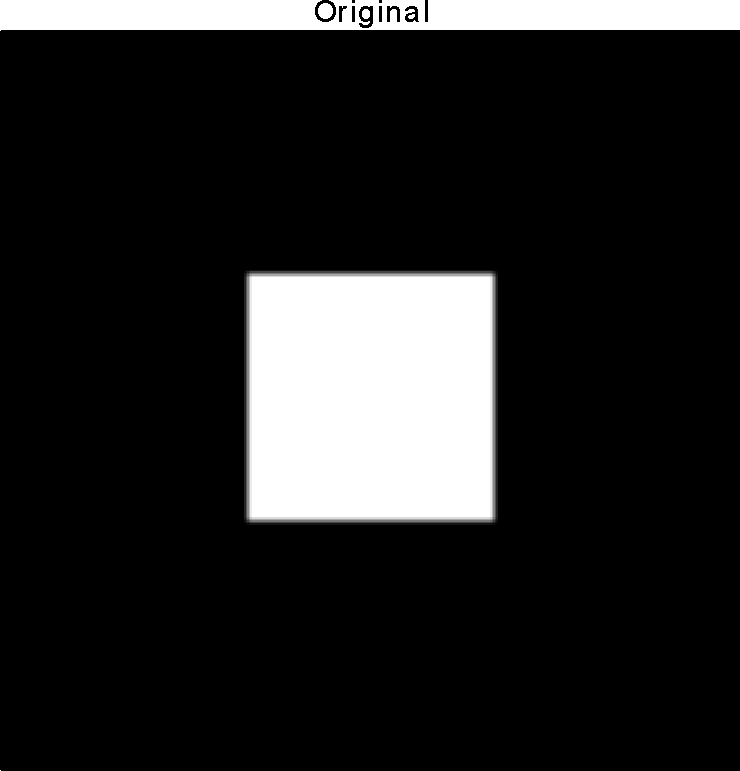
\includegraphics[width=.23\textwidth]{./figure/2D_White_Box_origin}
\label{fig:edge:01:origin} }
\subfigure[Gradient Magnitude]{
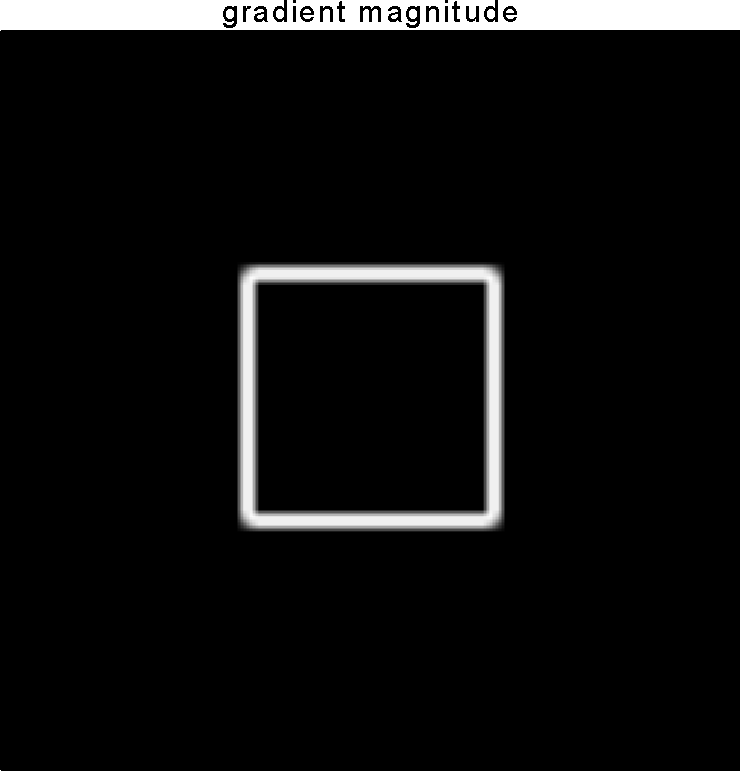
\includegraphics[width=.23\textwidth]{./figure/2D_White_Box_gradient_magnitude} 
\label{fig:edge:01:gradient_magnitude} }
\subfigure[Gradient Orientation]{
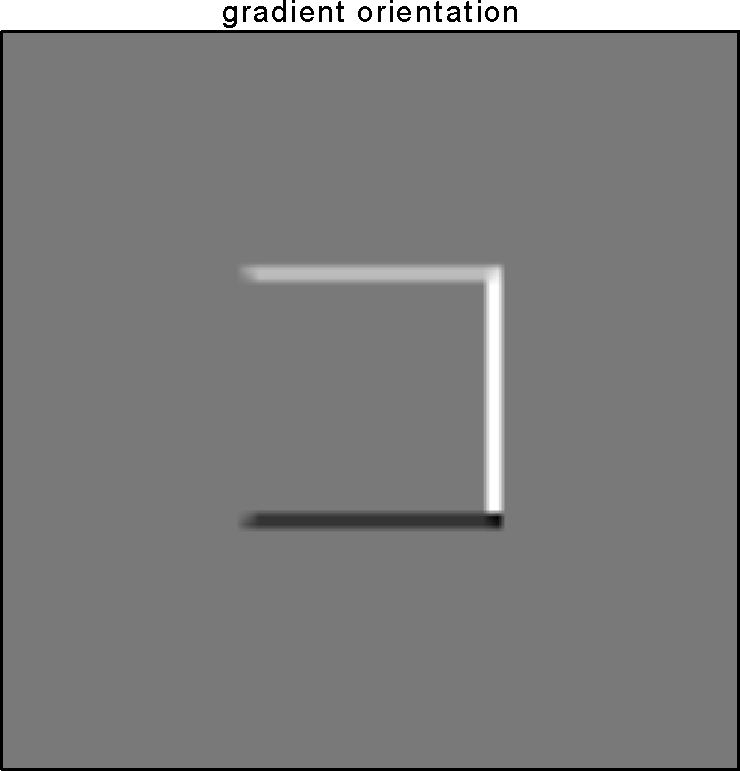
\includegraphics[width=.23\textwidth]{./figure/2D_White_Box_gradient_orientation}
\label{fig:edge:01:gradient_orientation} }
\subfigure[Laplacian]{
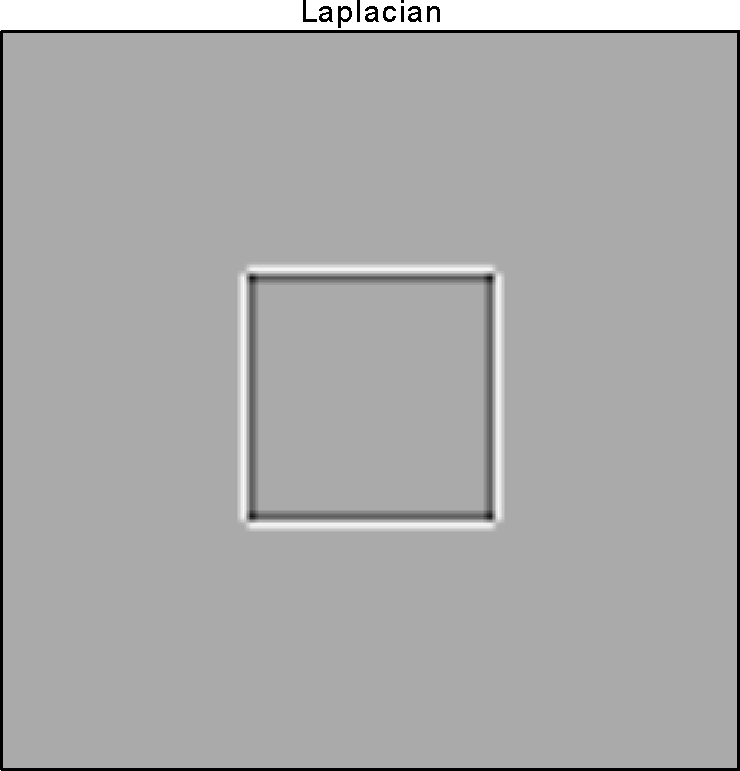
\includegraphics[width=.23\textwidth]{./figure/2D_White_Box_laplacian} 
\label{fig:edge:01:laplacian} }
\caption{Derivatives of \emph{2D\_White\_Box.pgm} by 1st order and 2nd order.}
\label{fig:edge:01}
\end{figure}

The clues for finding the edges are obtained from differential geometry.
Figure \ref{fig:edge:01} and Figure \ref{fig:edge:02} give the examples on 1st order and 2nd order derivatives.

\begin{figure}[h]
\centering
\subfigure[Origin]{
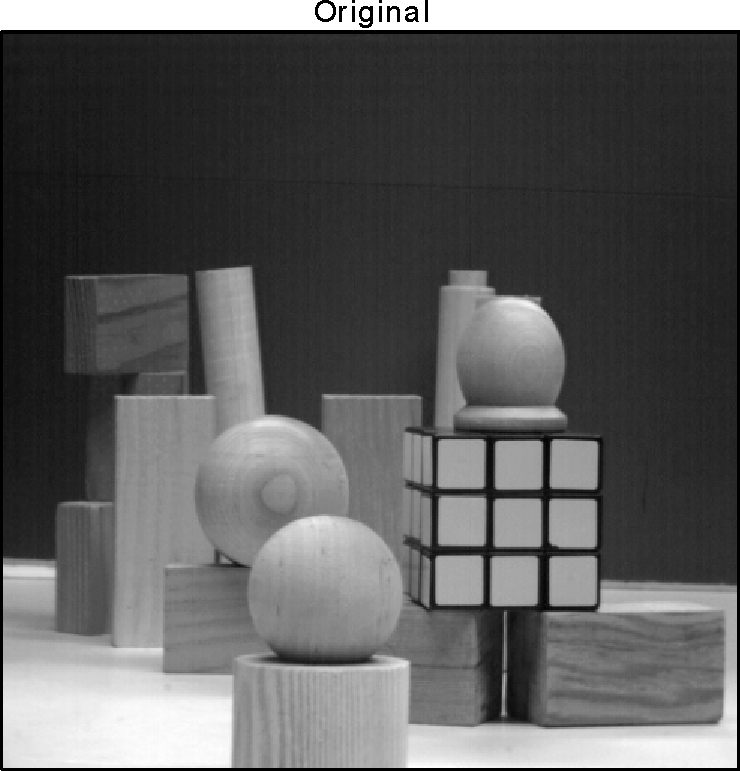
\includegraphics[width=.23\textwidth]{./figure/blocks_origin}
\label{fig:edge:02:origin} }
\subfigure[Gradient Magnitude]{
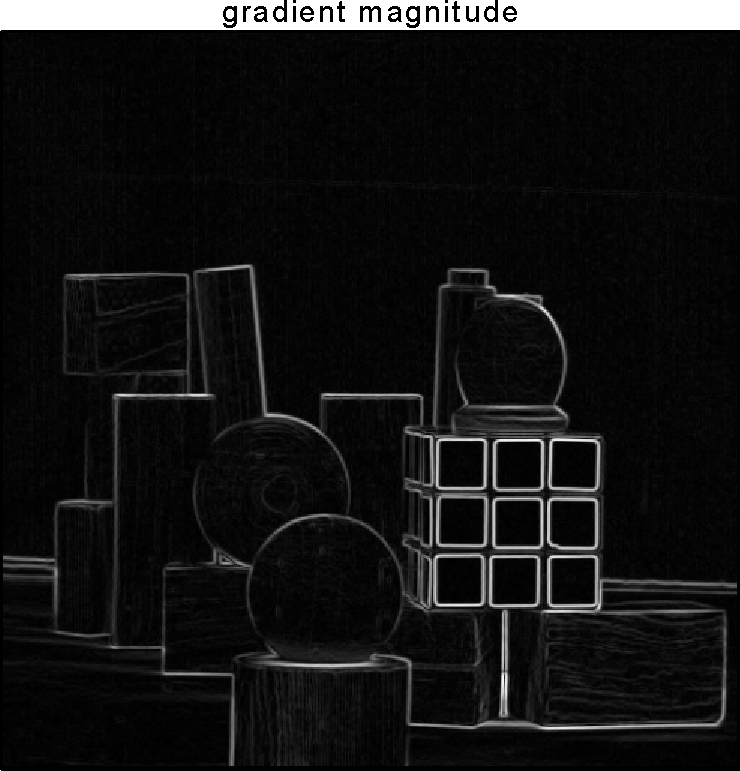
\includegraphics[width=.23\textwidth]{./figure/blocks_gradient_magnitude} 
\label{fig:edge:02:gradient_magnitude} } 
\subfigure[Gradient Orientation]{
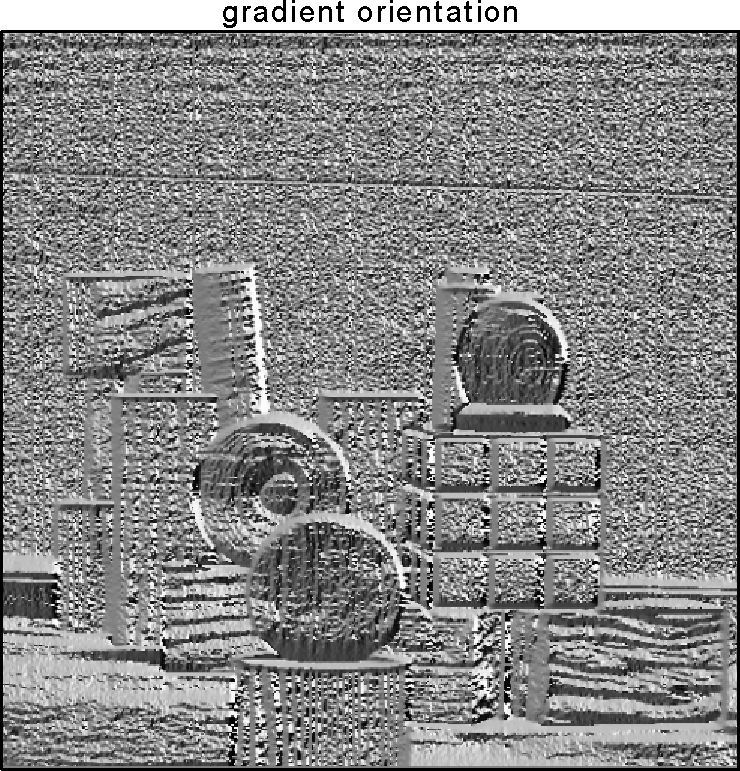
\includegraphics[width=.23\textwidth]{./figure/blocks_gradient_orientation}
\label{fig:edge:02:gradient_orientation} }
\subfigure[Laplacian]{
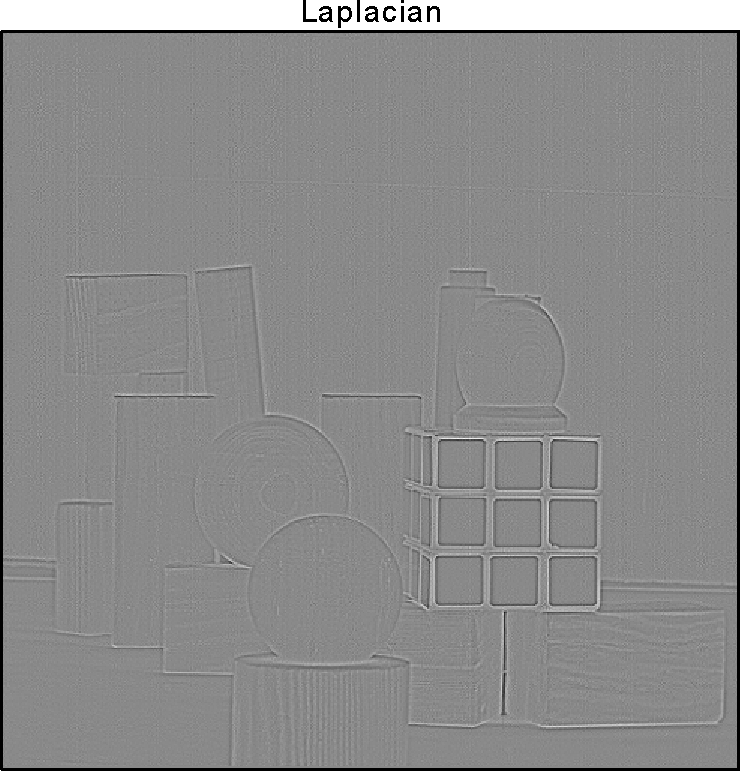
\includegraphics[width=.23\textwidth]{./figure/blocks_laplacian} 
\label{fig:edge:02:laplacian} }
\caption{Derivatives of \emph{blocks.pgm} by 1st order and 2nd order.}
\label{fig:edge:02}
\end{figure}

\subsection{edge detection}

\subsubsection{Canny edge detector}

\begin{figure}[h]
\centering
\subfigure[hi\_threshod=40, lo\_threshod=20]{
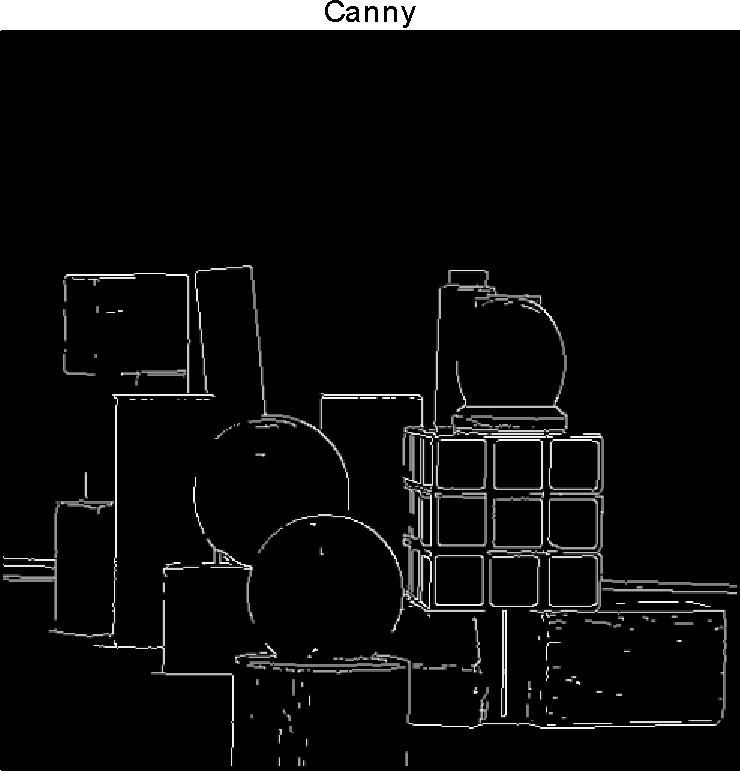
\includegraphics[width=.235\textwidth]{./figure/blocks_canny_20_40}
\label{fig:edge:02:canny:1} }
\subfigure[hi\_threshod=60, lo\_threshod=30]{
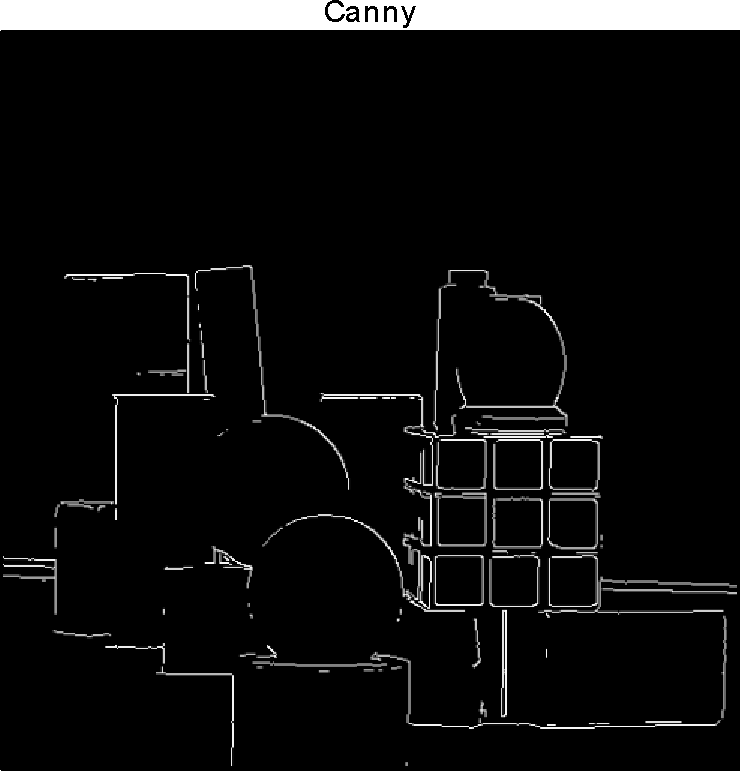
\includegraphics[width=.235\textwidth]{./figure/blocks_canny_30_60} 
\label{fig:edge:02:canny:2} } 
\subfigure[hi\_threshod=80, lo\_threshod=40]{
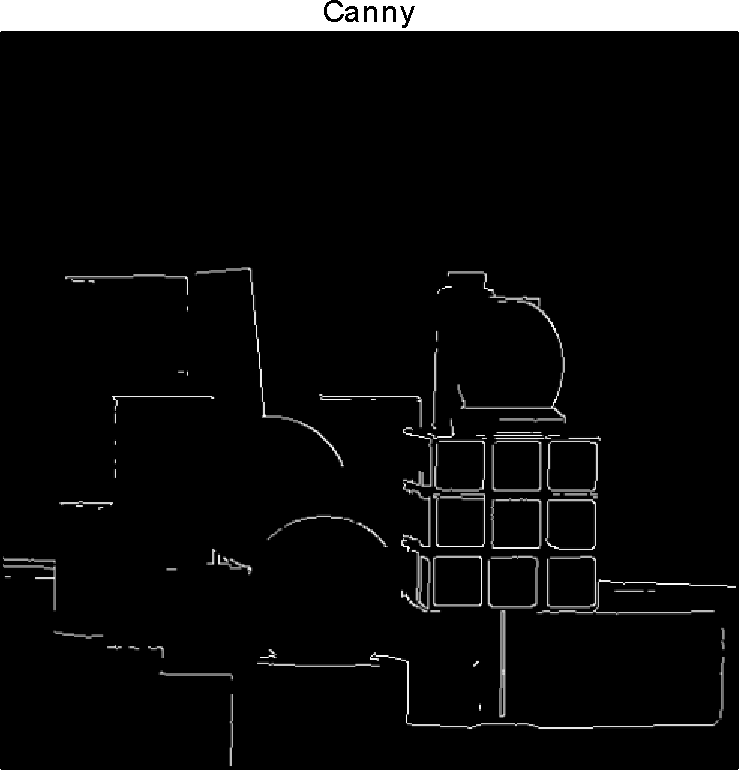
\includegraphics[width=.235\textwidth]{./figure/blocks_canny_40_80}
\label{fig:edge:02:canny:3} }
\subfigure[hi\_threshod=60, lo\_threshod=30, with Gaussian filter]{
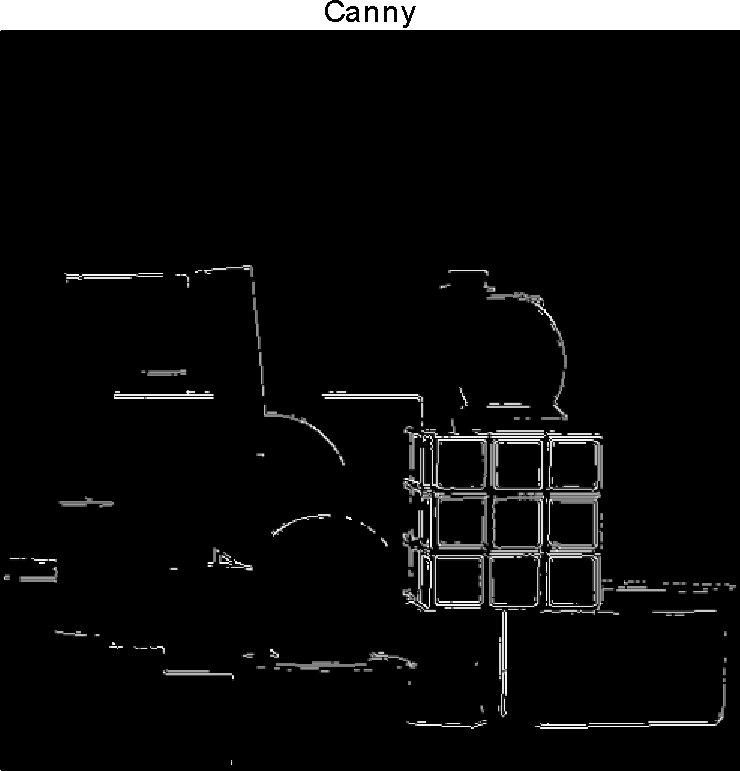
\includegraphics[width=.235\textwidth]{./figure/blocks_canny_gauss_30_60} 
\label{fig:edge:02:canny:gauss} }
\caption{Canny edge detector on \emph{blocks.pgm} using different parameters.}
\label{fig:edge:02:canny}
\end{figure}

\subsection{Laplacian zero-crossing edge detector}

\begin{figure}[h]
\centering
\subfigure[Threshold=40]{
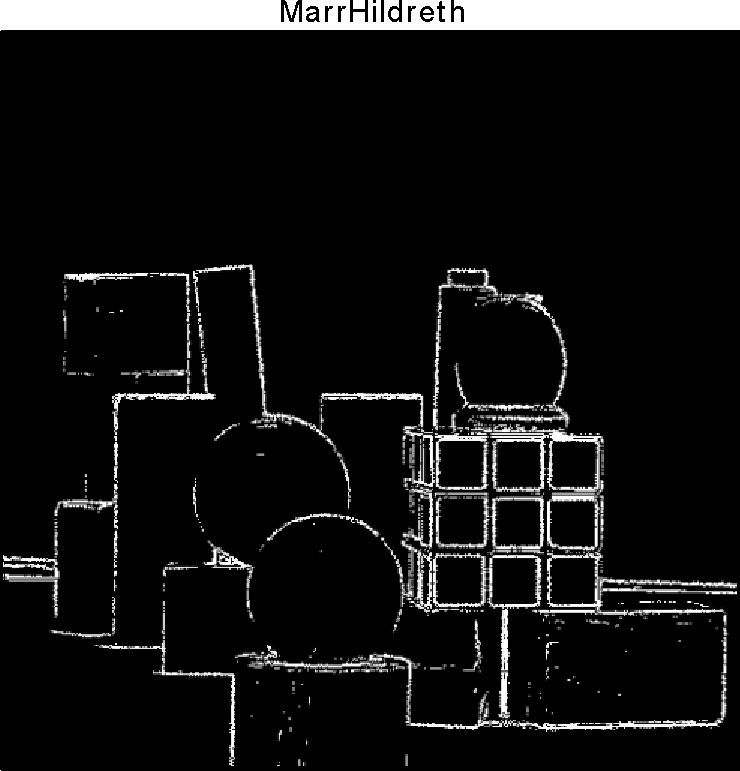
\includegraphics[width=.235\textwidth]{./figure/blocks_mh_40}
\label{fig:edge:02:mh:1} }
\subfigure[Threshold=60]{
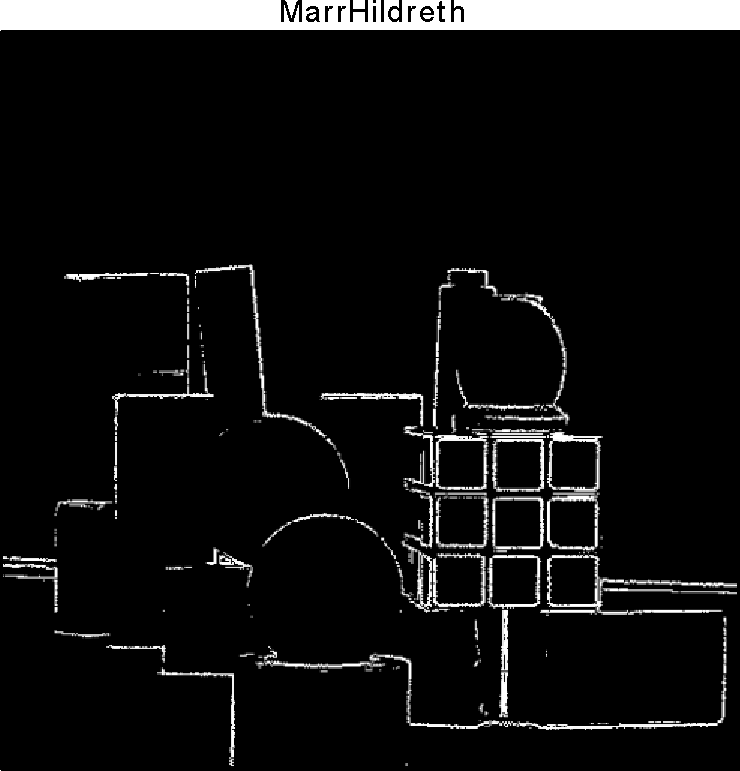
\includegraphics[width=.235\textwidth]{./figure/blocks_mh_60} 
\label{fig:edge:02:mh:2} } 
\subfigure[Threshold=80]{
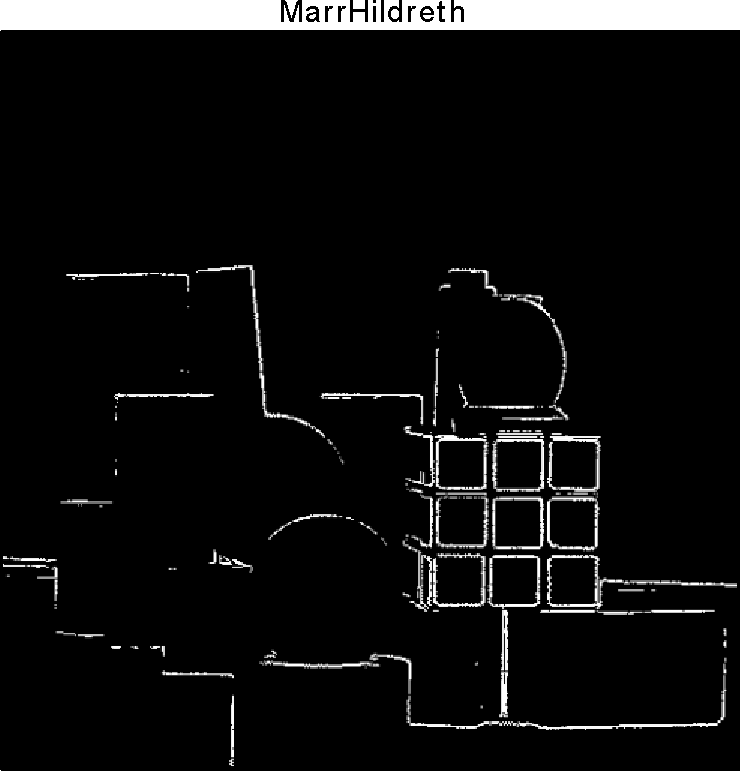
\includegraphics[width=.235\textwidth]{./figure/blocks_mh_80}
\label{fig:edge:02:mh:3} }
\subfigure[Threshold=40, with Gaussian filter]{
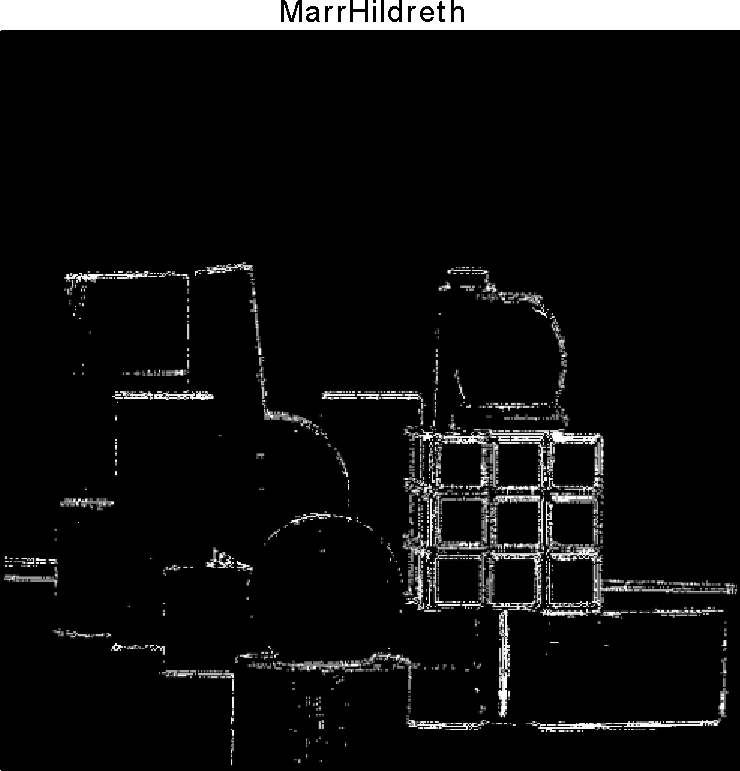
\includegraphics[width=.235\textwidth]{./figure/blocks_mh_gauss_40} 
\label{fig:edge:02:mh:gauss} }
\caption{Laplacian zero-crossing edge detector on \emph{blocks.pgm} using different parameters.}
\label{fig:edge:02:mh}
\end{figure}

\subsection{Conclusion}

\section{Hough transformation}

\subsection{Hough circle transformation}

\subsubsection{simple\_circle.pgm}

(124L, 127L)

\subsubsection{circles.ppm}

radius = 16
(89L, 115L)
(-7L, 122L)
(28L, 144L)
(28L, 149L)
(25L, 150L)
(90L, 196L)
(52L, 197L)

\begin{figure}[h]
\centering
\subfigure[Edges]{
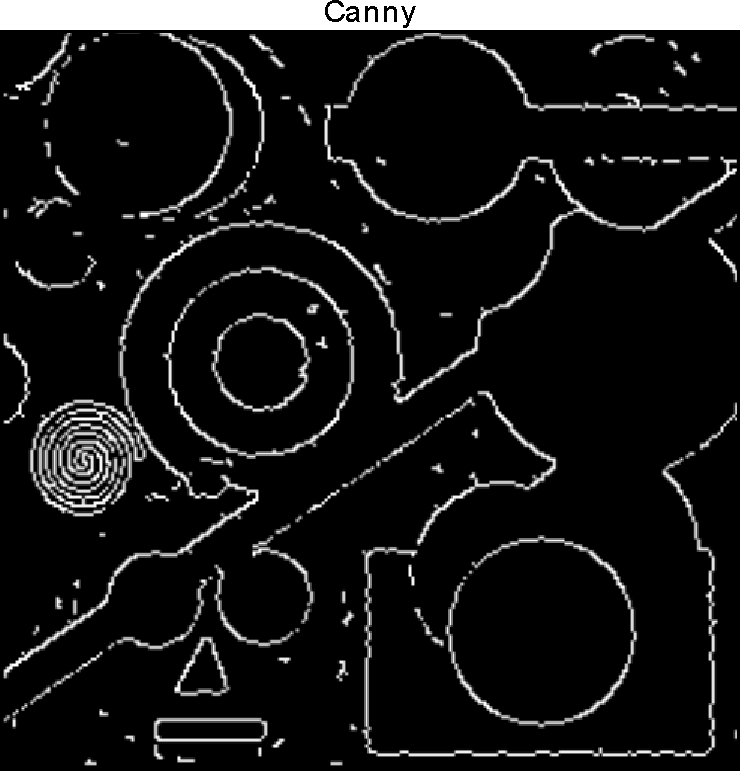
\includegraphics[width=.31\textwidth]{./figure/circles_ppm_canny_16}
\label{fig:hough:circle:16:edge} }
\subfigure[Hough space]{
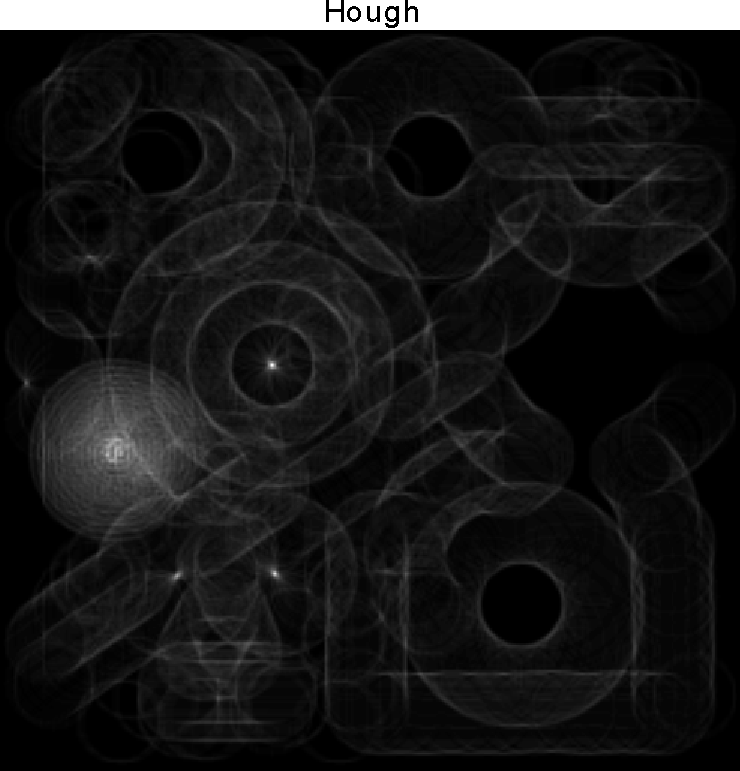
\includegraphics[width=.31\textwidth]{./figure/circles_ppm_hough_16} 
\label{fig:hough:circle:16:hough} } 
\subfigure[Circles found]{
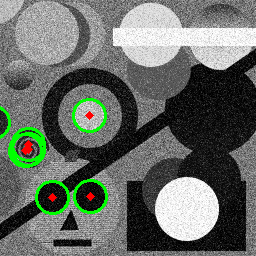
\includegraphics[width=.31\textwidth]{./figure/circles_ppm_circles_16}
\label{fig:hough:circle:16:circles} }
\caption{Detecting circles (radius=16) on \emph{circles.ppm}.}
\label{fig:hough:circle:16}
\end{figure}


radius = 32

(46L, 32L)
(57L, 34L)
(150L, 34L)
(220L, 37L)
(158L, 67L)
(79L, 102L)
(89L, 115L)
(173L, 189L)
(186L, 208L)

\begin{figure}[h]
\centering
\subfigure[Edges]{
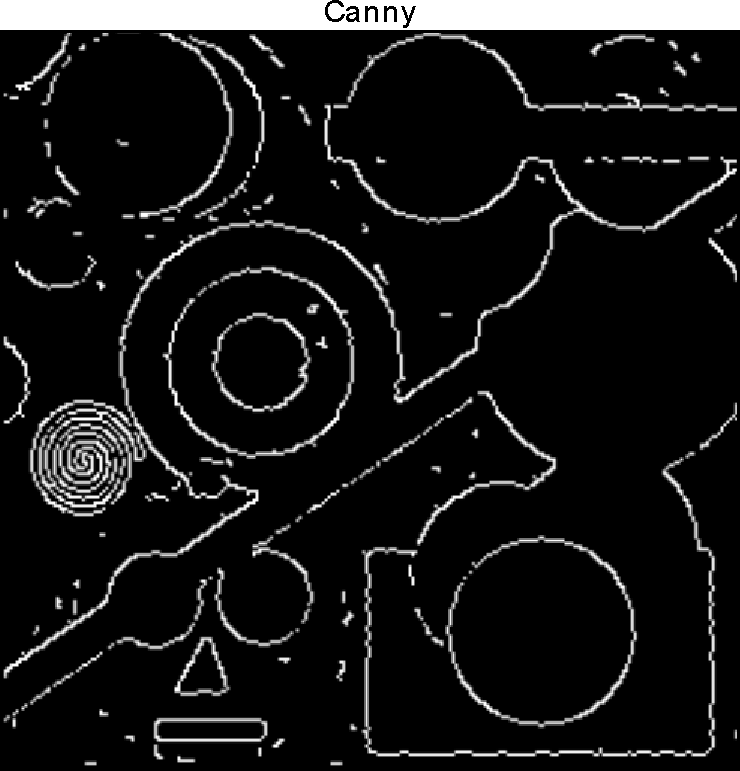
\includegraphics[width=.31\textwidth]{./figure/circles_ppm_canny_32}
\label{fig:hough:circle:32:edge} }
\subfigure[Hough space]{
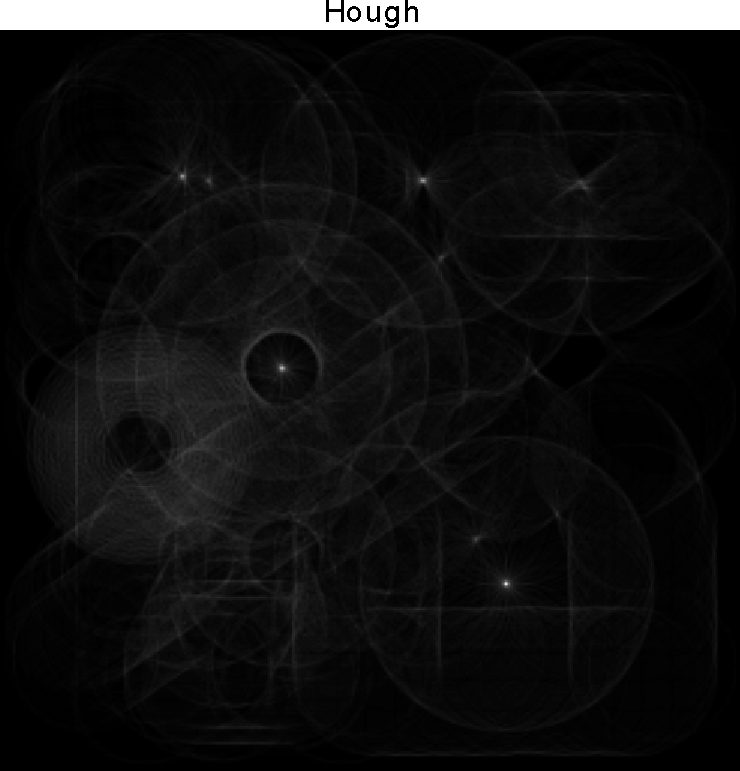
\includegraphics[width=.31\textwidth]{./figure/circles_ppm_hough_32} 
\label{fig:hough:circle:32:hough} } 
\subfigure[Circles found]{
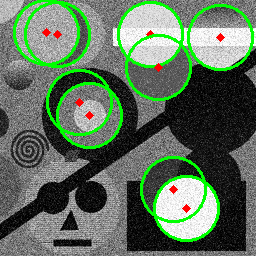
\includegraphics[width=.31\textwidth]{./figure/circles_ppm_circles_32}
\label{fig:hough:circle:32:circles} }
\caption{Detecting circles (radius=32) on \emph{circles.ppm}.}
\label{fig:hough:circle:32}
\end{figure}

radius = 64

(0L, 103L)
(0L, 108L)
(89L, 115L)
(71L, 206L)

\begin{figure}[h]
\centering
\subfigure[Edges]{
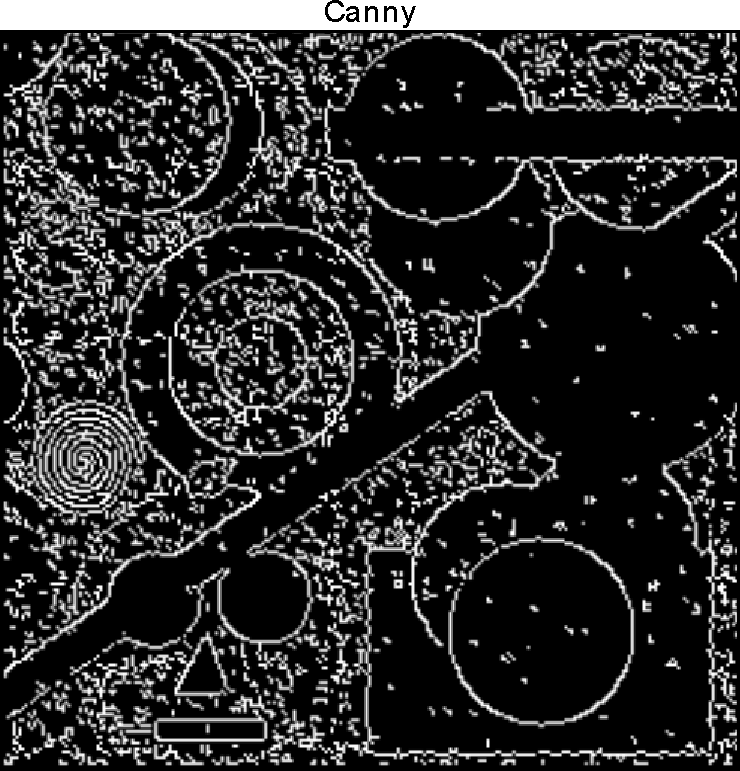
\includegraphics[width=.31\textwidth]{./figure/circles_ppm_canny_48}
\label{fig:hough:circle:48:edge} }
\subfigure[Hough space]{
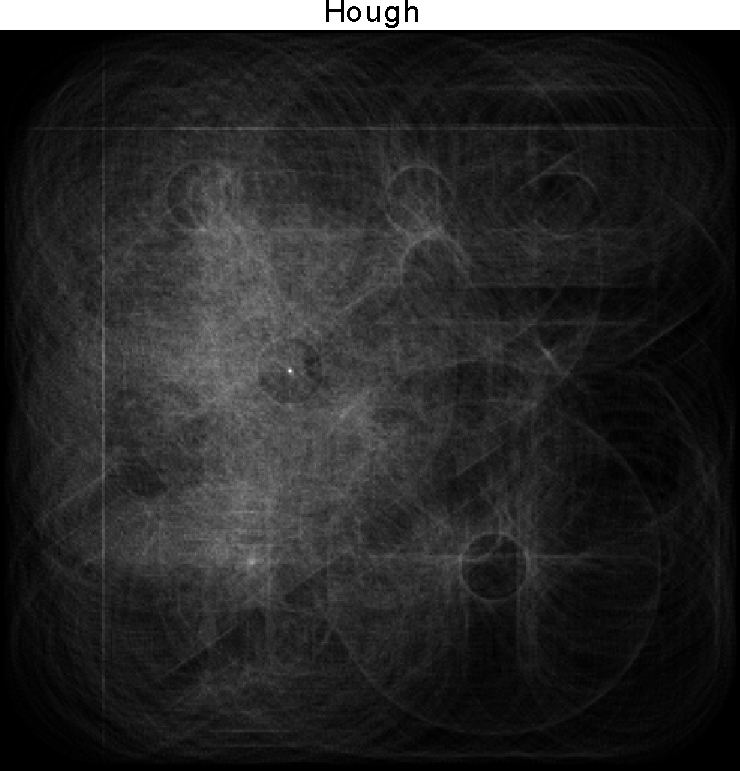
\includegraphics[width=.31\textwidth]{./figure/circles_ppm_hough_48} 
\label{fig:hough:circle:48:hough} } 
\subfigure[Circles found]{
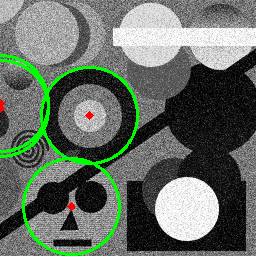
\includegraphics[width=.31\textwidth]{./figure/circles_ppm_circles_48}
\label{fig:hough:circle:48:circles} }
\caption{Detecting circles (radius=32) on \emph{circles.ppm}.}
\label{fig:hough:circle:48}
\end{figure}

Different rules for margin 

radius = 32
(-7L, -8L)
(200L, -4L)
(150L, 34L)
(220L, 37L)
(158L, 67L)
(199L, 116L)
(208L, 178L)
(173L, 189L)
(186L, 208L)

\begin{figure}[h]
\centering
\subfigure[Edges]{
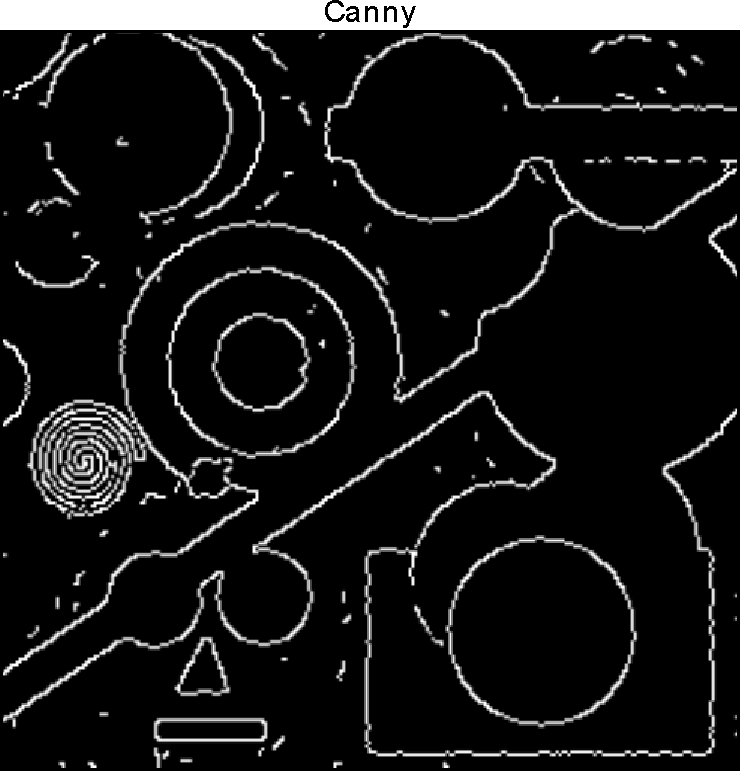
\includegraphics[width=.31\textwidth]{./figure/circles_ppm_canny_32_cv}
\label{fig:hough:circle:32:cv:edge} }
\subfigure[Hough space]{
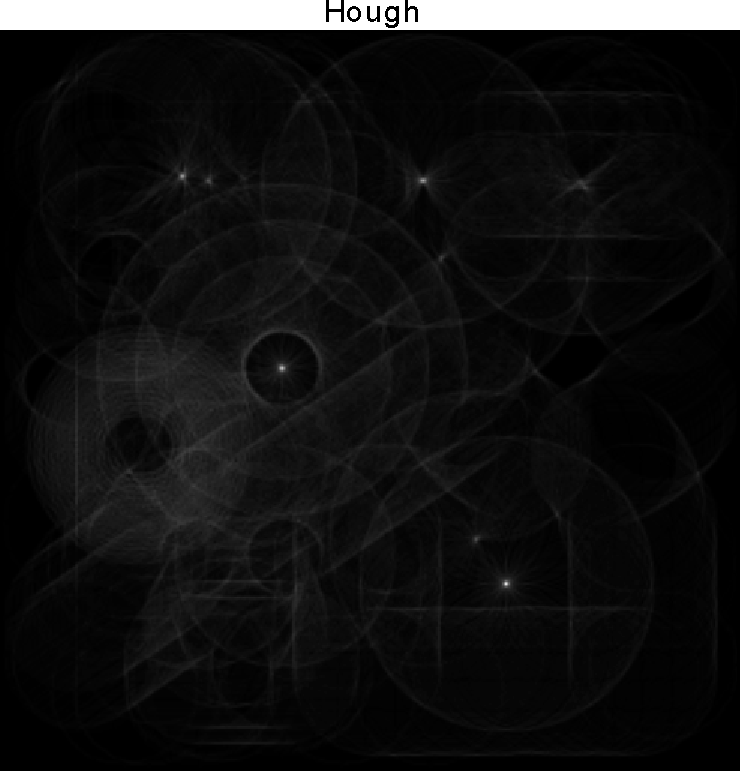
\includegraphics[width=.31\textwidth]{./figure/circles_ppm_hough_32_cv} 
\label{fig:hough:circle:32:cv:hough} } 
\subfigure[Circles found]{
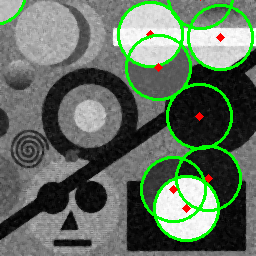
\includegraphics[width=.31\textwidth]{./figure/circles_ppm_circles_32_cv}
\label{fig:hough:circle:32:cv:circles} }
\caption{Detecting circles (radius=32) on \emph{circles.ppm}.}
\label{fig:hough:circle:32:cv}
\end{figure}

Weighted revote


\subsection{Conclusion}



\end{document}